%% template.tex
%% from
%% bare_conf.tex
%% V1.4b
%% 2015/08/26
%% by Michael Shell
%% See:
%% http://www.michaelshell.org/
%% for current contact information.
%%
%% This is a skeleton file demonstrating the use of IEEEtran.cls
%% (requires IEEEtran.cls version 1.8b or later) with an IEEE
%% conference paper.
%%
%% Support sites:
%% http://www.michaelshell.org/tex/ieeetran/
%% http://www.ctan.org/pkg/ieeetran
%% and
%% http://www.ieee.org/

%%*************************************************************************
%% Legal Notice:
%% This code is offered as-is without any warranty either expressed or
%% implied; without even the implied warranty of MERCHANTABILITY or
%% FITNESS FOR A PARTICULAR PURPOSE!
%% User assumes all risk.
%% In no event shall the IEEE or any contributor to this code be liable for
%% any damages or losses, including, but not limited to, incidental,
%% consequential, or any other damages, resulting from the use or misuse
%% of any information contained here.
%%
%% All comments are the opinions of their respective authors and are not
%% necessarily endorsed by the IEEE.
%%
%% This work is distributed under the LaTeX Project Public License (LPPL)
%% ( http://www.latex-project.org/ ) version 1.3, and may be freely used,
%% distributed and modified. A copy of the LPPL, version 1.3, is included
%% in the base LaTeX documentation of all distributions of LaTeX released
%% 2003/12/01 or later.
%% Retain all contribution notices and credits.
%% ** Modified files should be clearly indicated as such, including  **
%% ** renaming them and changing author support contact information. **
%%*************************************************************************


% *** Authors should verify (and, if needed, correct) their LaTeX system  ***
% *** with the testflow diagnostic prior to trusting their LaTeX platform ***
% *** with production work. The IEEE's font choices and paper sizes can   ***
% *** trigger bugs that do not appear when using other class files.       ***                          ***
% The testflow support page is at:
% http://www.michaelshell.org/tex/testflow/

\documentclass[conference,final,]{IEEEtran}
% Some Computer Society conferences also require the compsoc mode option,
% but others use the standard conference format.
%
% If IEEEtran.cls has not been installed into the LaTeX system files,
% manually specify the path to it like:
% \documentclass[conference]{../sty/IEEEtran}





% Some very useful LaTeX packages include:
% (uncomment the ones you want to load)


% *** MISC UTILITY PACKAGES ***
%
%\usepackage{ifpdf}
% Heiko Oberdiek's ifpdf.sty is very useful if you need conditional
% compilation based on whether the output is pdf or dvi.
% usage:
% \ifpdf
%   % pdf code
% \else
%   % dvi code
% \fi
% The latest version of ifpdf.sty can be obtained from:
% http://www.ctan.org/pkg/ifpdf
% Also, note that IEEEtran.cls V1.7 and later provides a builtin
% \ifCLASSINFOpdf conditional that works the same way.
% When switching from latex to pdflatex and vice-versa, the compiler may
% have to be run twice to clear warning/error messages.






% *** CITATION PACKAGES ***
%
%\usepackage{cite}
% cite.sty was written by Donald Arseneau
% V1.6 and later of IEEEtran pre-defines the format of the cite.sty package
% \cite{} output to follow that of the IEEE. Loading the cite package will
% result in citation numbers being automatically sorted and properly
% "compressed/ranged". e.g., [1], [9], [2], [7], [5], [6] without using
% cite.sty will become [1], [2], [5]--[7], [9] using cite.sty. cite.sty's
% \cite will automatically add leading space, if needed. Use cite.sty's
% noadjust option (cite.sty V3.8 and later) if you want to turn this off
% such as if a citation ever needs to be enclosed in parenthesis.
% cite.sty is already installed on most LaTeX systems. Be sure and use
% version 5.0 (2009-03-20) and later if using hyperref.sty.
% The latest version can be obtained at:
% http://www.ctan.org/pkg/cite
% The documentation is contained in the cite.sty file itself.






% *** GRAPHICS RELATED PACKAGES ***
%
\ifCLASSINFOpdf
  % \usepackage[pdftex]{graphicx}
  % declare the path(s) where your graphic files are
  % \graphicspath{{../pdf/}{../jpeg/}}
  % and their extensions so you won't have to specify these with
  % every instance of \includegraphics
  % \DeclareGraphicsExtensions{.pdf,.jpeg,.png}
\else
  % or other class option (dvipsone, dvipdf, if not using dvips). graphicx
  % will default to the driver specified in the system graphics.cfg if no
  % driver is specified.
  % \usepackage[dvips]{graphicx}
  % declare the path(s) where your graphic files are
  % \graphicspath{{../eps/}}
  % and their extensions so you won't have to specify these with
  % every instance of \includegraphics
  % \DeclareGraphicsExtensions{.eps}
\fi
% graphicx was written by David Carlisle and Sebastian Rahtz. It is
% required if you want graphics, photos, etc. graphicx.sty is already
% installed on most LaTeX systems. The latest version and documentation
% can be obtained at:
% http://www.ctan.org/pkg/graphicx
% Another good source of documentation is "Using Imported Graphics in
% LaTeX2e" by Keith Reckdahl which can be found at:
% http://www.ctan.org/pkg/epslatex
%
% latex, and pdflatex in dvi mode, support graphics in encapsulated
% postscript (.eps) format. pdflatex in pdf mode supports graphics
% in .pdf, .jpeg, .png and .mps (metapost) formats. Users should ensure
% that all non-photo figures use a vector format (.eps, .pdf, .mps) and
% not a bitmapped formats (.jpeg, .png). The IEEE frowns on bitmapped formats
% which can result in "jaggedy"/blurry rendering of lines and letters as
% well as large increases in file sizes.
%
% You can find documentation about the pdfTeX application at:
% http://www.tug.org/applications/pdftex





% *** MATH PACKAGES ***
%
%\usepackage{amsmath}
% A popular package from the American Mathematical Society that provides
% many useful and powerful commands for dealing with mathematics.
%
% Note that the amsmath package sets \interdisplaylinepenalty to 10000
% thus preventing page breaks from occurring within multiline equations. Use:
%\interdisplaylinepenalty=2500
% after loading amsmath to restore such page breaks as IEEEtran.cls normally
% does. amsmath.sty is already installed on most LaTeX systems. The latest
% version and documentation can be obtained at:
% http://www.ctan.org/pkg/amsmath





% *** SPECIALIZED LIST PACKAGES ***
%
%\usepackage{algorithmic}
% algorithmic.sty was written by Peter Williams and Rogerio Brito.
% This package provides an algorithmic environment fo describing algorithms.
% You can use the algorithmic environment in-text or within a figure
% environment to provide for a floating algorithm. Do NOT use the algorithm
% floating environment provided by algorithm.sty (by the same authors) or
% algorithm2e.sty (by Christophe Fiorio) as the IEEE does not use dedicated
% algorithm float types and packages that provide these will not provide
% correct IEEE style captions. The latest version and documentation of
% algorithmic.sty can be obtained at:
% http://www.ctan.org/pkg/algorithms
% Also of interest may be the (relatively newer and more customizable)
% algorithmicx.sty package by Szasz Janos:
% http://www.ctan.org/pkg/algorithmicx




% *** ALIGNMENT PACKAGES ***
%
%\usepackage{array}
% Frank Mittelbach's and David Carlisle's array.sty patches and improves
% the standard LaTeX2e array and tabular environments to provide better
% appearance and additional user controls. As the default LaTeX2e table
% generation code is lacking to the point of almost being broken with
% respect to the quality of the end results, all users are strongly
% advised to use an enhanced (at the very least that provided by array.sty)
% set of table tools. array.sty is already installed on most systems. The
% latest version and documentation can be obtained at:
% http://www.ctan.org/pkg/array


% IEEEtran contains the IEEEeqnarray family of commands that can be used to
% generate multiline equations as well as matrices, tables, etc., of high
% quality.




% *** SUBFIGURE PACKAGES ***
%\ifCLASSOPTIONcompsoc
%  \usepackage[caption=false,font=normalsize,labelfont=sf,textfont=sf]{subfig}
%\else
%  \usepackage[caption=false,font=footnotesize]{subfig}
%\fi
% subfig.sty, written by Steven Douglas Cochran, is the modern replacement
% for subfigure.sty, the latter of which is no longer maintained and is
% incompatible with some LaTeX packages including fixltx2e. However,
% subfig.sty requires and automatically loads Axel Sommerfeldt's caption.sty
% which will override IEEEtran.cls' handling of captions and this will result
% in non-IEEE style figure/table captions. To prevent this problem, be sure
% and invoke subfig.sty's "caption=false" package option (available since
% subfig.sty version 1.3, 2005/06/28) as this is will preserve IEEEtran.cls
% handling of captions.
% Note that the Computer Society format requires a larger sans serif font
% than the serif footnote size font used in traditional IEEE formatting
% and thus the need to invoke different subfig.sty package options depending
% on whether compsoc mode has been enabled.
%
% The latest version and documentation of subfig.sty can be obtained at:
% http://www.ctan.org/pkg/subfig




% *** FLOAT PACKAGES ***
%

%\usepackage{fixltx2e}
% fixltx2e, the successor to the earlier fix2col.sty, was written by
% Frank Mittelbach and David Carlisle. This package corrects a few problems
% in the LaTeX2e kernel, the most notable of which is that in current
% LaTeX2e releases, the ordering of single and double column floats is not
% guaranteed to be preserved. Thus, an unpatched LaTeX2e can allow a
% single column figure to be placed prior to an earlier double column
% figure.
% Be aware that LaTeX2e kernels dated 2015 and later have fixltx2e.sty's
% corrections already built into the system in which case a warning will
% be issued if an attempt is made to load fixltx2e.sty as it is no longer
% needed.
% The latest version and documentation can be found at:
% http://www.ctan.org/pkg/fixltx2e


%\usepackage{stfloats}
% stfloats.sty was written by Sigitas Tolusis. This package gives LaTeX2e
% the ability to do double column floats at the bottom of the page as well
% as the top. (e.g., "\begin{figure*}[!b]" is not normally possible in
% LaTeX2e). It also provides a command:
%\fnbelowfloat
% to enable the placement of footnotes below bottom floats (the standard
% LaTeX2e kernel puts them above bottom floats). This is an invasive package
% which rewrites many portions of the LaTeX2e float routines. It may not work
% with other packages that modify the LaTeX2e float routines. The latest
% version and documentation can be obtained at:
% http://www.ctan.org/pkg/stfloats
% Do not use the stfloats baselinefloat ability as the IEEE does not allow
% \baselineskip to stretch. Authors submitting work to the IEEE should note
% that the IEEE rarely uses double column equations and that authors should try
% to avoid such use. Do not be tempted to use the cuted.sty or midfloat.sty
% packages (also by Sigitas Tolusis) as the IEEE does not format its papers in
% such ways.
% Do not attempt to use stfloats with fixltx2e as they are incompatible.
% Instead, use Morten Hogholm'a dblfloatfix which combines the features
% of both fixltx2e and stfloats:
%
% \usepackage{dblfloatfix}
% The latest version can be found at:
% http://www.ctan.org/pkg/dblfloatfix




% *** PDF, URL AND HYPERLINK PACKAGES ***
%
%\usepackage{url}
% url.sty was written by Donald Arseneau. It provides better support for
% handling and breaking URLs. url.sty is already installed on most LaTeX
% systems. The latest version and documentation can be obtained at:
% http://www.ctan.org/pkg/url
% Basically, \url{my_url_here}.




% *** Do not adjust lengths that control margins, column widths, etc. ***
% *** Do not use packages that alter fonts (such as pslatex).         ***
% There should be no need to do such things with IEEEtran.cls V1.6 and later.
% (Unless specifically asked to do so by the journal or conference you plan
% to submit to, of course. )



%% BEGIN MY ADDITIONS %%


\usepackage{graphicx}
% We will generate all images so they have a width \maxwidth. This means
% that they will get their normal width if they fit onto the page, but
% are scaled down if they would overflow the margins.
\makeatletter
\def\maxwidth{\ifdim\Gin@nat@width>\linewidth\linewidth
\else\Gin@nat@width\fi}
\makeatother
\let\Oldincludegraphics\includegraphics
\renewcommand{\includegraphics}[1]{\Oldincludegraphics[width=\maxwidth]{#1}}

\usepackage[unicode=true]{hyperref}

\hypersetup{
            pdftitle={Bare Demo of IEEEtran.cls for IEEE Conferences},
            pdfkeywords={keyword 1, keyword 2},
            pdfborder={0 0 0},
            breaklinks=true}
\urlstyle{same}  % don't use monospace font for urls

% Pandoc toggle for numbering sections (defaults to be off)
\setcounter{secnumdepth}{0}

% Pandoc syntax highlighting


% Pandoc header

\providecommand{\tightlist}{%
  \setlength{\itemsep}{0pt}\setlength{\parskip}{0pt}}

%% END MY ADDITIONS %%


\hyphenation{op-tical net-works semi-conduc-tor}

\begin{document}
%
% paper title
% Titles are generally capitalized except for words such as a, an, and, as,
% at, but, by, for, in, nor, of, on, or, the, to and up, which are usually
% not capitalized unless they are the first or last word of the title.
% Linebreaks \\ can be used within to get better formatting as desired.
% Do not put math or special symbols in the title.
\title{Bare Demo of IEEEtran.cls for IEEE Conferences}

% author names and affiliations
% use a multiple column layout for up to three different
% affiliations

\author{

%% ---- classic IEEETrans wide authors' list ----------------
 % -- end affiliation.wide
%% ----------------------------------------------------------



%% ---- classic IEEETrans one column per institution --------
 %% -- beg if/affiliation.institution-columnar
\IEEEauthorblockN{
  %% -- beg for/affiliation.institution.author
Cristian Camilo Gañan %% -- end for/affiliation.institution.author
}
\IEEEauthorblockA{Departamento de Ciencias Forestales\\
Universidad Nacional de Colombia\\
Medelín, Antioquia
\\ccganant@unal.edu.co
}
\and
\IEEEauthorblockN{
  %% -- beg for/affiliation.institution.author
Camilo Andres Cruz Sanchez %% -- end for/affiliation.institution.author
}
\IEEEauthorblockA{Departamento de Ciencias Forestales\\
Universidad Nacional de Colombia\\
Medellín, Antioquia
\\cacruzs@unal.edu.co
}
\and
\IEEEauthorblockN{
  %% -- beg for/affiliation.institution.author
Juan Pablo Caicedo Garcia %% -- end for/affiliation.institution.author
}
\IEEEauthorblockA{Departamento de Ciencias Forestales\\
Universidad Nacional de Colombia\\
Medellín, Antioquia
  %% -- beg for/affiliation.institution.author
\\jpcaicedog@unal.edu.co
 %% -- end for/affiliation.institution.author
}
 %% -- end for/affiliation.institution
 %% -- end if/affiliation.institution-columnar
%% ----------------------------------------------------------





%% ---- one column per author, classic/default IEEETrans ----
 %% -- end if/affiliation.institution-columnar
%% ----------------------------------------------------------

}

% conference papers do not typically use \thanks and this command
% is locked out in conference mode. If really needed, such as for
% the acknowledgment of grants, issue a \IEEEoverridecommandlockouts
% after \documentclass

% for over three affiliations, or if they all won't fit within the width
% of the page, use this alternative format:
%
%\author{\IEEEauthorblockN{Michael Shell\IEEEauthorrefmark{1},
%Homer Simpson\IEEEauthorrefmark{2},
%James Kirk\IEEEauthorrefmark{3},
%Montgomery Scott\IEEEauthorrefmark{3} and
%Eldon Tyrell\IEEEauthorrefmark{4}}
%\IEEEauthorblockA{\IEEEauthorrefmark{1}School of Electrical and Computer Engineering\\
%Georgia Institute of Technology,
%Atlanta, Georgia 30332--0250\\ Email: see http://www.michaelshell.org/contact.html}
%\IEEEauthorblockA{\IEEEauthorrefmark{2}Twentieth Century Fox, Springfield, USA\\
%Email: homer@thesimpsons.com}
%\IEEEauthorblockA{\IEEEauthorrefmark{3}Starfleet Academy, San Francisco, California 96678-2391\\
%Telephone: (800) 555--1212, Fax: (888) 555--1212}
%\IEEEauthorblockA{\IEEEauthorrefmark{4}Tyrell Inc., 123 Replicant Street, Los Angeles, California 90210--4321}}




% use for special paper notices
%\IEEEspecialpapernotice{(Invited Paper)}




% make the title area
\maketitle

% As a general rule, do not put math, special symbols or citations
% in the abstract
\begin{abstract}
The abstract goes here. On multiple lines eventually.
\end{abstract}

% keywords
\begin{IEEEkeywords}
keyword 1; keyword 2
\end{IEEEkeywords}

% use for special paper notices



% make the title area
\maketitle

% no keywords

% For peer review papers, you can put extra information on the cover
% page as needed:
% \ifCLASSOPTIONpeerreview
% \begin{center} \bfseries EDICS Category: 3-BBND \end{center}
% \fi
%
% For peerreview papers, this IEEEtran command inserts a page break and
% creates the second title. It will be ignored for other modes.
\IEEEpeerreviewmaketitle


\hypertarget{introducciuxf3n}{%
\section{Introducción}\label{introducciuxf3n}}

\onecolumn[]

Los estudios de diversidad han sido catalogados desde el punto de vista
científico como una ayuda enorme para entender la dinámica de los
distintos ecosistemas, también como sinónimo de ``variedad de vida''
(1). Existen dos áreas principales en las cuales los estudios y medidas
de diversidad han tenido una gran aplicación, se pueden ver entonces
desde el punto de vista de la conservación la cual está basada en que
las comunidades ricas en especies son mejores que las pobres en estas, y
desde el punto de vista de la supervisión ambiental donde se tienen en
cuenta los efectos adversos en la reducción de la diversidad o en un
cambio de forma de la distribución de abundancia de las especies (2). En
los agrosistemas mantener o restaurar altos niveles de diversidad,
aumenta su resistencia al cambio climático, apoya la provisión
equilibrada de servicios ecosistémicos y contribuye a la conectividad
del hábitat (3). La diversidad como una medida tangible es obtenida por
medio de diversos índices que además de dar un valor de la diversidad en
cualquier comunidad también expresa comportamientos en las comunidades
tales como la riqueza, dominancia, la equidad, la abundancia relativa,
similitud y disimilitud, entre otros(4). Por otra parte, Robert H.
Whittaker (1972)(5) formalizó matemáticamente el concepto de diversidad
de especies y planteó tres componentes cuantificables: alfa (α), beta
(β) y gamma (γ), los cuales son importantes a la hora de querer conocer
y diferenciar la diversidad y estructura de distintas comunidades, los
índices alfa han sido importantes en conocer la diversidad dentro de una
comunidad (En este caso parcela), los beta para conocer y comparar la
diversidad entre varias comunidades y corroborar el reemplazamiento de
especies entre una comunidad y otra (En el caso del estudio parcelas),
generalmente, la diversidad alfa se evalúa con la riqueza de especies
presentes en una comunidad y la diversidad beta con índices que miden la
disimilitud en la composición de especies entre las comunidades (7).

La importancia de la determinación de los diferentes índices, está en
diferenciar entre tipos de bosques y conocer los diferentes cambios
ambientales para explicar el reemplazamiento de especies y el cambio en
la estructura de los mismos, se entiende que la estructura de los
bosques está relacionada con la diversidad, pero también con condiciones
ambientales como el clima y el suelo(8), y que dicha estructura tiende a
responder a las exigencias de las especies(10) que hacen que esta cambie
continuamente(9), entonces conocer las diferentes diversidades de estos
tipos de bosques y compararlas da una idea acerca de qué tan diversos
son y cual de ellos representa una mayor complejidad estructural
teniendo en cuenta su diversidad y factores bióticos y abióticos que la
controlan. La estructura

\hypertarget{muxe9todos}{%
\section{Métodos}\label{muxe9todos}}

\hypertarget{resultados-y-discusiuxf3n}{%
\section{Resultados y discusión}\label{resultados-y-discusiuxf3n}}

\begin{table}

\caption{\label{tab:unnamed-chunk-2}indices alfa}
\centering
\begin{tabular}[t]{l|r|r|r|r}
\hline
Parcela & Margalef & Shannon & Simpson & Fisher\\
\hline
62 & 0.2227848 & 0.0616067 & 0.0222194 & 2.042935\\
\hline
69 & 1.1476553 & 1.1471140 & 0.6213018 & 6.370040\\
\hline
70 & 0.5824134 & 0.3795349 & 0.1789802 & 3.945655\\
\hline
\end{tabular}
\end{table}

\begin{verbatim}
## # A tibble: 1 x 3
##   `62-69` `62-70` `69-70`
##     <dbl>   <dbl>   <dbl>
## 1       0       0       0
\end{verbatim}

\begin{verbatim}
##     1   2
## 2 0.0    
## 3 0.8 0.0
\end{verbatim}

\begin{verbatim}
## [1] 13.66667
\end{verbatim}

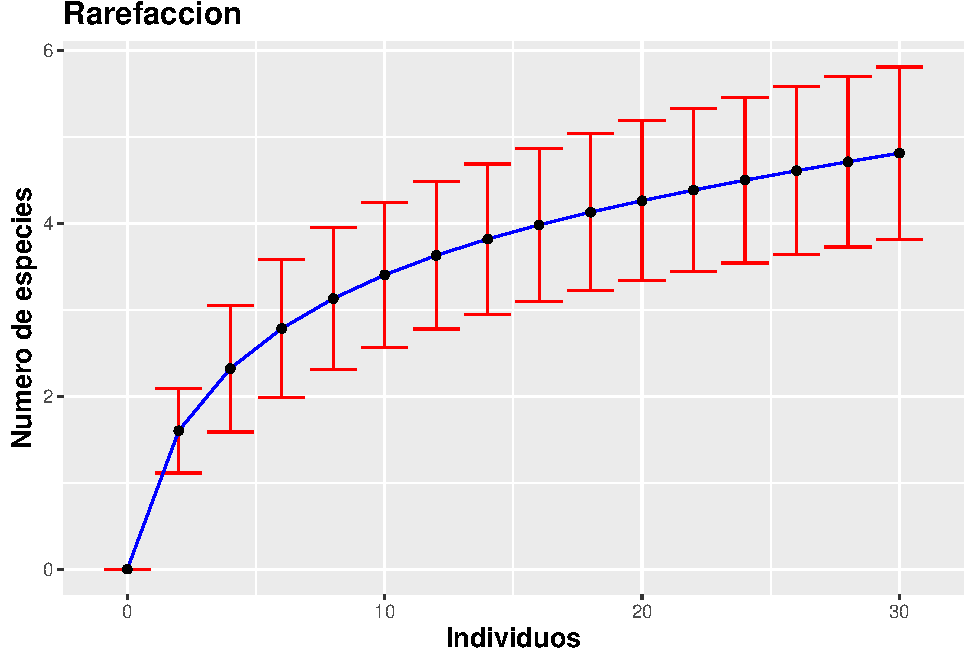
\includegraphics{mangrove_files/figure-latex/unnamed-chunk-4-1.pdf}

\begin{verbatim}
## # A tibble: 9 x 5
##   Especie                        DR     AR    FR    IVI
##   <fct>                       <dbl>  <dbl> <dbl>  <dbl>
## 1 Laguncularia racemosa      1.93    1.52  18.2   21.6 
## 2 Montrichardia arborescens  6.96   17.7    9.09  33.7 
## 3 Pachira cf. aquatica       4.52    3.54   9.09  17.1 
## 4 Pelliciera rhizophorae     0.159   0.505  9.09   9.76
## 5 Prioria copaifera          0.0740  0.505  9.09   9.67
## 6 Pterocarpus officinalis   41.5    16.2    9.09  66.8 
## 7 Raphia taedigera           7.12    1.01   9.09  17.2 
## 8 Rhizophora mangle         37.5    58.6   18.2  114.  
## 9 Tabebuia chrysantha        0.214   0.505  9.09   9.81
\end{verbatim}

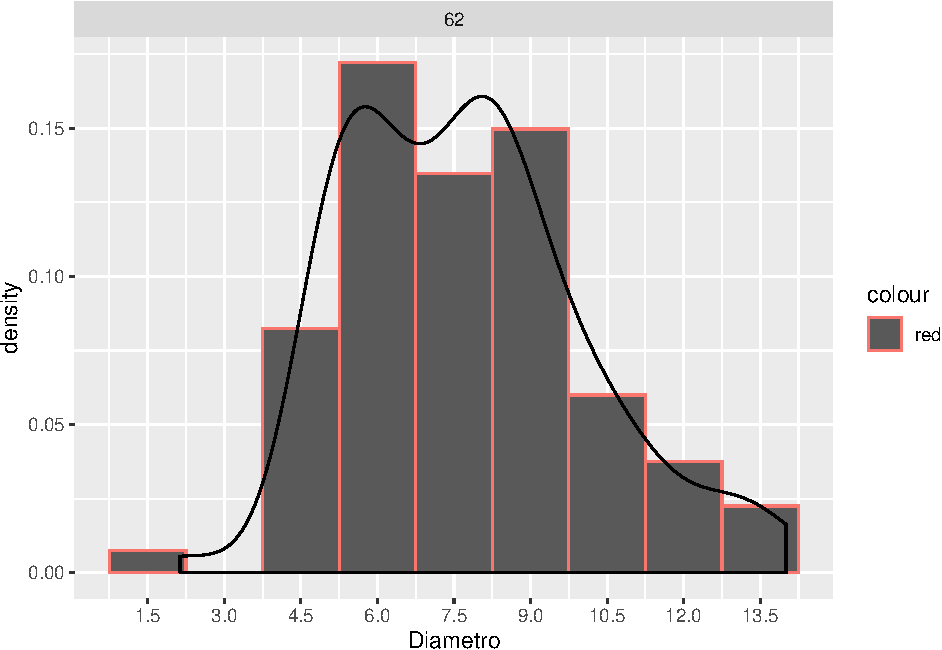
\includegraphics{mangrove_files/figure-latex/unnamed-chunk-6-1.pdf}
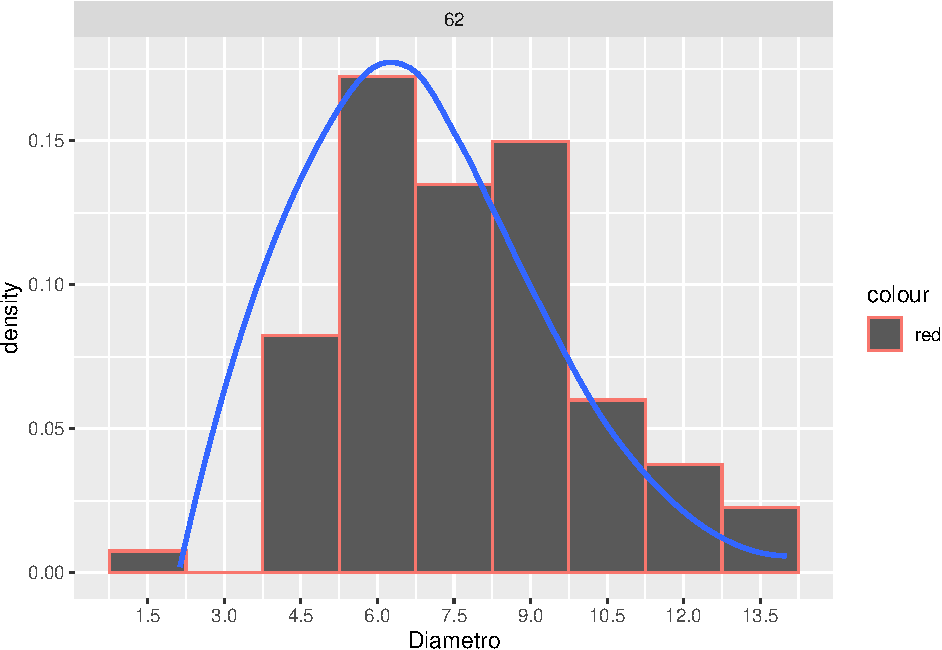
\includegraphics{mangrove_files/figure-latex/unnamed-chunk-6-2.pdf}

\begin{verbatim}
## 
##  Shapiro-Wilk normality test
## 
## data:  datam$Count
## W = 0.79812, p-value = 0.008887
\end{verbatim}

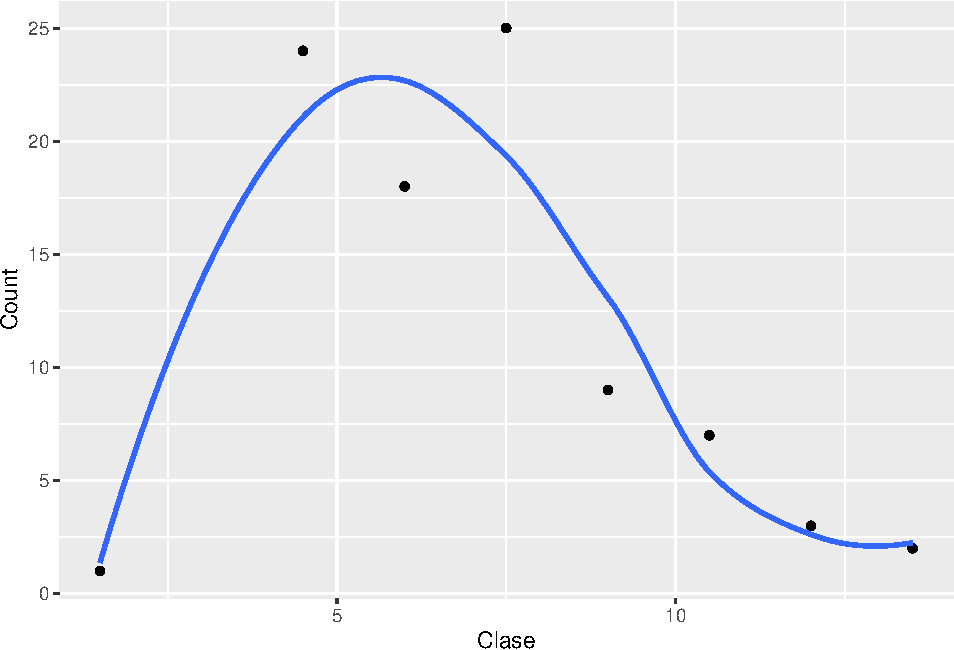
\includegraphics{mangrove_files/figure-latex/unnamed-chunk-6-3.pdf}
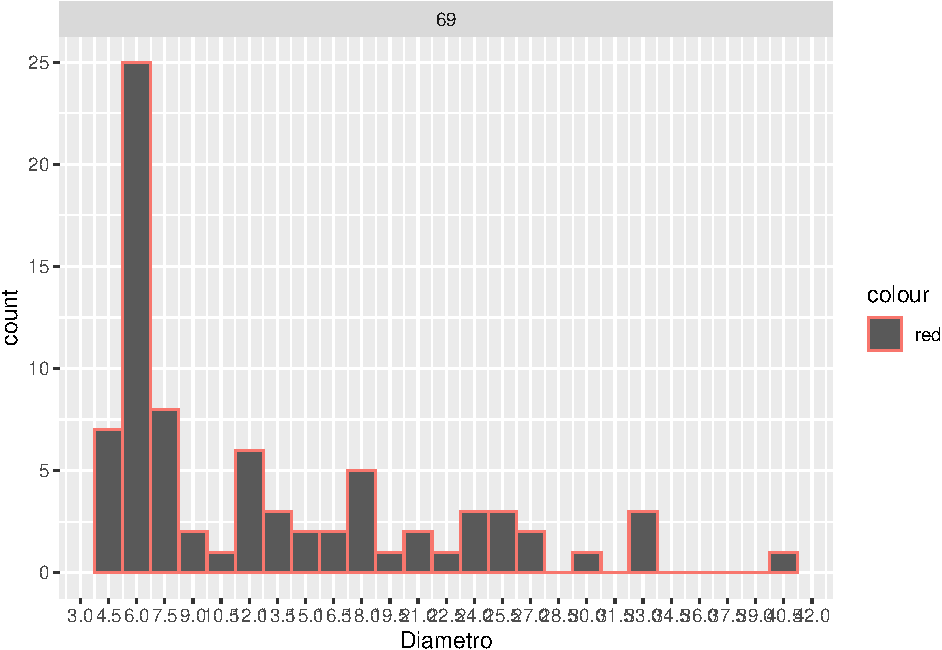
\includegraphics{mangrove_files/figure-latex/unnamed-chunk-6-4.pdf}
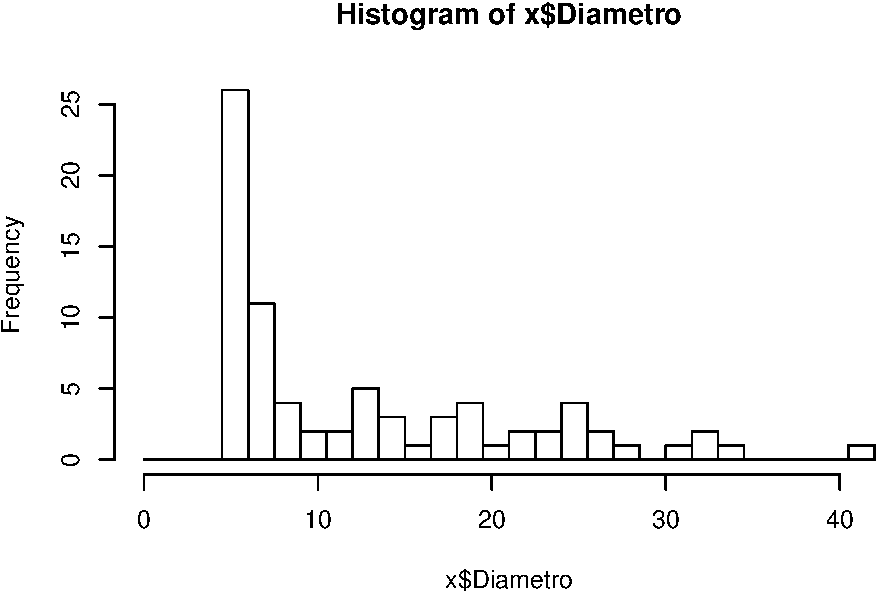
\includegraphics{mangrove_files/figure-latex/unnamed-chunk-6-5.pdf}
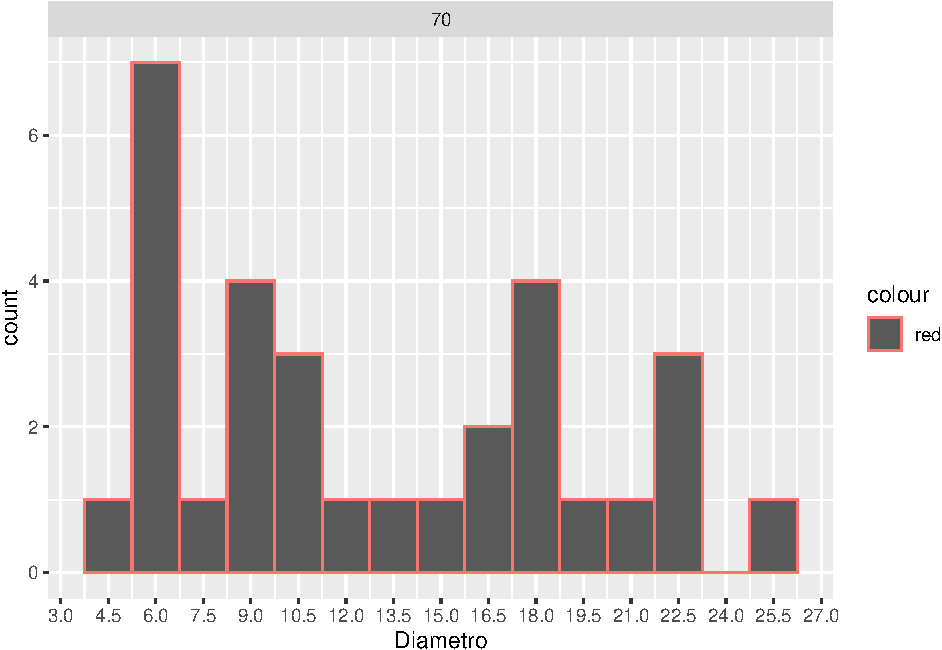
\includegraphics{mangrove_files/figure-latex/unnamed-chunk-6-6.pdf}
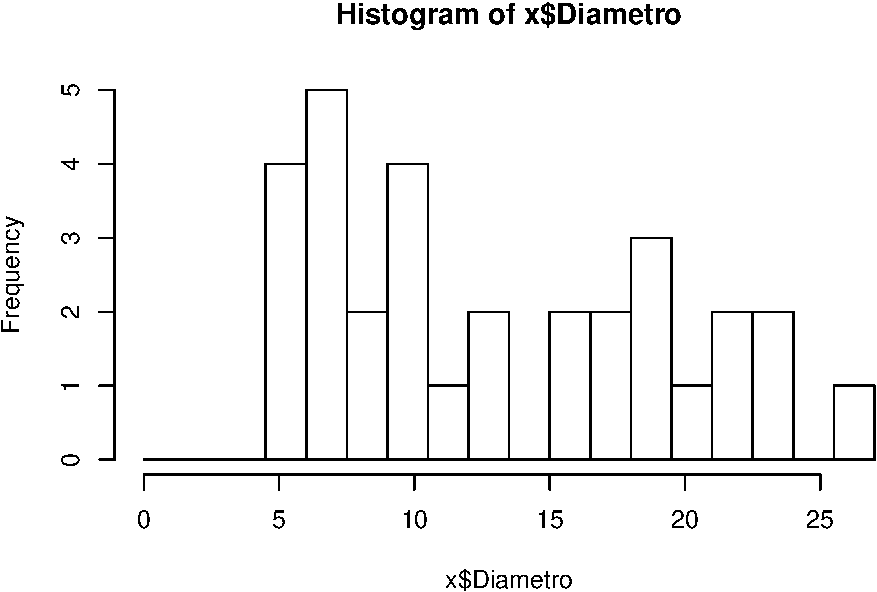
\includegraphics{mangrove_files/figure-latex/unnamed-chunk-6-7.pdf}

\end{document}


